\documentclass[a4paper,french,bookmarks]{article}

\usepackage{./Structure/4PE18TEXTB}

\newboxans
\usepackage{booktabs}

\begin{document}

    \renewcommand{\thesection}{\Roman{section}} 
    \renewcommand{\thesubsection}{\thesection.\Alph{subsection}}
    \setlist[enumerate]{font=\color{white5!60!black}\bfseries\sffamily}
    \renewcommand{\labelenumi}{\thesection.\arabic{enumi}.}
    \renewcommand*{\labelenumii}{\thesection.\arabic{enumi}.\alph{enumii}.}
    
    \stylizeDocSpe{Physique}{Devoir maison n° 3}{}{Pour le mardi 4 octobre 2022}
    
    \section{Premier problème}
    
    \subsection{Échantillonneur bloqueur (numérique)}
    
    Un signal numérique est moins sensible aux perturbations qu'un signal analogique et surtout, il se prête bien plus facilement au traitement (numérique !). Pour ces raisons, on choisit de convertir le signal analogique issu du détecteur en signal numérique binaire. La chaîne de transmission des données est représentée figure \ref{fig:fig1}.
    %
    \begin{center}
        \begin{minipage}{0.8\linewidth}
            \centering
            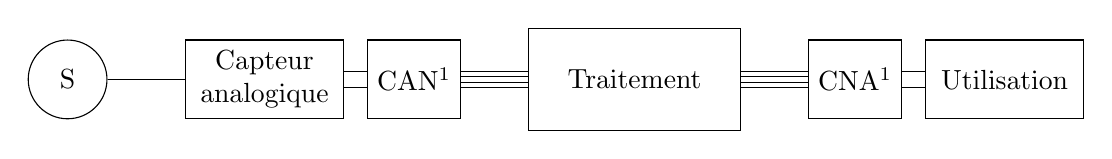
\begin{tikzpicture}
                \node[draw,circle,minimum size=1cm] (S) at (0,0) {S};
                \node[draw,rectangle,minimum size=1cm,align=center,minimum  width=2cm] (CA) at (2.5,0) {Capteur\\ analogique};
                \node[draw,rectangle,minimum size=1cm,align=center] (CAN) at (4.4,0) {CAN\footnotemark[1]};
                
                \node[draw,rectangle,minimum size=1cm,align=center,minimum  width=2.7cm,minimum height=1.3cm] (T) at (7.2,0) {Traitement};
                
                \node[draw,rectangle,minimum size=1cm,align=center] (CNA) at (10,0) {CNA\footnotemark[1]};
                
                \node[draw,rectangle,minimum size=1cm,align=center,minimum  width=2cm] (U) at (11.9,0) {Utilisation};
                
                \draw (S) -- (CA);
                
                \draw[transform canvas={yshift=3pt}] (CA) -- (CAN);
                \draw[transform canvas={yshift=-3pt}] (CA) -- (CAN);
                
                \draw[transform canvas={yshift=3pt}] (CAN) -- (T);
                \draw[transform canvas={yshift=1pt}] (CAN) -- (T);
                \draw[transform canvas={yshift=-1pt}] (CAN) -- (T);
                \draw[transform canvas={yshift=-3pt}] (CAN) -- (T);
                
                \draw[transform canvas={yshift=3pt}] (T) -- (CNA);
                \draw[transform canvas={yshift=1pt}] (T) -- (CNA);
                \draw[transform canvas={yshift=-1pt}] (T) -- (CNA);
                \draw[transform canvas={yshift=-3pt}] (T) -- (CNA);
                
                \draw[transform canvas={yshift=3pt}] (CNA) -- (U);
                \draw[transform canvas={yshift=-3pt}] (CNA) -- (U);
            \end{tikzpicture}
            \renewcommand{\thempfootnote}{\arabic{mpfootnote}}
            \footnotetext[1]{CAN = Convertisseur Analogique Numérique / CNA = Convertisseur Numérique Analogique}
        \end{minipage}
        %
        \text{}\\[2pt]
        %
        \begin{minipage}{0.9\linewidth}
            \captionof{figure}{Chaîne de traitement du signal. La boîte \textnormal{Capteur analogique} peut contenir des éléments de traitement analogique.}
	        \label{fig:fig1}
        \end{minipage}
    \end{center}
    %
    La conversion analogique numérique commence par l'échantillonnage, transformation du signal continu analogique en signal discontinu. L'élément réalisant cette transformation (figure \ref{fig:fig2}) est essentiellement un interrupteur commandé par une tension périodique $e\p{t}$ de fréquence $f_\text e= \sfrac{1}{T_\text e}$ ($T_\text e$ étant la période de fermeture de l'interrupteur). La durée de fermeture est très petite devant $T_\text e$.\medskip
    
    Le signal de commande $e\p{t}$ est modélisé par une suite périodique de pics d'amplitude constante et de largeur temporelle $\epsilon$ très petite devant $T_\text e$ (voir figure \ref{fig:fig3}) ; le pic centré sur l'instant $t = nT_\text e$ étant noté $\delta\p{t - nT_\text e}$, la tension s'exprime alors par
    %
    \[ e\p{t} = \sum_{n=0}^{\infty} \delta\p{t - nT_\text e} \]
    %
    \begin{center}
        \begin{minipage}{0.8\linewidth}
            \centering
            \begin{circuitikz}
                \draw (-1, 0) node[eground] {} to[vsource, v_=$e\p{t}$] ++(0, 2) --++(0, 0.7) --++(3, 0);
                
                \draw[short, -{Triangle}] (2, 2.7) --++(0, -0.5) node[label={[font=\footnotesize]north east:$K_C$}] {};
                
                \draw (1, 0) node[eground] {} to[vsource, v_=$V\p{t}$] ++(0, 2)  --++(0.75, 0) to[nos] ++(0.5, 0) --++(0.75, 0) to[R,l=$R_\text u$] ++(0, -2) node[eground] {};
                
                \draw[dashed] (1.6, 3) --++(1.2,0) --++(0, -1.2) --++(-1.2, 0) --++(0, 1.2);
                
                \draw[] (4.5, 1.5) to[short] ++(0.5, 0) node[label={[font=\footnotesize]north:$K_C$}] {} to[nos] ++(0.5, 0) node[] {$\qquad\qquad\iff$};
                
                \node (e) at (7.1, 2) {$e\p{t}$};
                \node[draw,rectangle,align=center] (M) at (8.5,2) {$\times$};
                \node (v) at (8.5, 1) {$V\p{t}$};
                \node (s) at (11, 2) {$v_\text e\p{t} = K_0e\p{t}V\p{t}$};
                
                \draw (e) -- (M);
                \draw (v) -- (M);
                \draw (s) -- (M);
                
                \draw[dashed] (4.25, 2.6) --++(8.5,0) --++(0, -2) --++(-8.5, 0) --++(0, 2);
            \end{circuitikz}
        \end{minipage}
        %
        \text{}\\[2pt]
        %
        \begin{minipage}{0.9\linewidth}
            \captionof{figure}{Principe d'un échantillonneur. Le commutateur $K_C$ est un multiplieur commandé de gain $K_0$ entre $e\p{t}$ et le signal $V\p{t}$. Le circuit d'utilisation est modélisé par la résistance $R_u$.}
	        \label{fig:fig2}
        \end{minipage}
    \end{center}
    %
    \begin{center}
        \begin{minipage}{0.8\linewidth}
            \centering
            \resizebox{\linewidth}{!}{\includegraphics[]{dm3fig/dm3fig3.png}}
        \end{minipage}
        %
        %
        \text{}\\[2pt]
        %
        \begin{minipage}{0.9\linewidth}
            \captionof{figure}{Échantillonage. Le cartouche en haut à droite donne l'allure de $v_\text e\p{t}$, tension aux bornes de $R_u$ ; l'allure de la courbe originale est préservée, mais le pointé du sommet est imprécis.}
	        \label{fig:fig3}
        \end{minipage}
    \end{center}
    
    \begin{enumerate}
        \item Que peut-on dire sur le spectre de $v_\text e\p{t}$ par rapport à celui de $V\p{t}$ ? En déduire une condition sur le choix de $T_\text e$ si l'on souhaite qu'il n'y ait pas de perte d'information entre $v_\text e\p{t}$ et $V\p{t}$.
        
        \noafter
        %
        \boxans{
            On a $V_\text e\p{t} = K_0e\p{t}V\p{t}$. On a $e\p{t}$ pérodique, de pulsation $2\pi f_\text e$, donc en décomposant en série de \textsc{Fourier} :
            %
            \[ e\p{t} = e_0 + \sum_{k=1}^{+\infty} e_k\cos{2\pi nf_\text et + \varphi_k} \qquad\text{donc}\qquad v_\text e \p{t} = K_0e_0V\p{t} + \sum_{k=1}^{+\infty} K_0e_kV\p{t}\cos{2\pi nf_\text et + \varphi_k}\]
            %
            Puisque $V\p{t}$ peut-être vu comme une somme/intégrale de signaux sinusoïdaux, par distributivité et linéarité on peut considérer $V\p{t}$ de forme sinusoïdale de fréquence $f_\text V$ : \quad $V\p{t} = V_0\cos{2\pi f_\text Vt + \phi}$.
            %
            \[ v_\text e\p{t} = K_0V_0e_0\cos{2\pi f_Vt + \phi} + \sum_{k=1}^{+\infty} \dfrac{K_0V_0e_k}{2}\intc{\cos{2\pi t\p{nf_\text e - f_\text V} + \varphi_k - \psi} +\vphantom{\int_a^b} \cos{2\pi t\p{nf_\text e + f_\text V} + \varphi_k + \psi}}\]
            %
            Ainsi le spectre de $v_\text e\p{t}$ contient une harmonique en $f_\text V$, et pour chaque $k \in \bdN^*$, une harmonique en $nf_\text e - f_\text V$ et une en $nf_\text e + f_\text V$. Plus généralement, le spectre de $v_\text e\p{t}$ sera de la forme :
            %
        }
        %
        \nobefore
        %
        \boxansconc{
            \begin{center}
                \begin{tikzpicture}
                    \begin{axis}[
                       clip                =   false,
                        axis lines          =   middle,
                        minor tick num      =   4,
                        domain              =   0:53,
                        %xtick distance      =   1,
                        %ytick distance      =   1,
                        trig format plots   =   rad,
                        trig format         =   rad,
                        xlabel              =   {$f$ (Hz)},
                        ylabel              =   {Amplitude (dB)},
                        xmin                =   0,
                        xmax                =   53,
                        ymin                =   0,
                        ymax                =   5,
                        width               =   15cm,
                        height              =   6cm,
                        grid                =   none,
                        xtick               =   {20, 40},
                        ytick               =   {},
                        xticklabels         =   {$\color{main5}f_\text e$, $\color{main7}2f_\text e$},
                        yticklabels         =   {}
                    ]
                        \addplot[color=main3,samples=500,thick]{1/2*abs( cos(2*abs(x)) + 3*sin(2.2*abs(x)) + 2*sin(3*abs(x))*cos(7*abs(x)) + 6 )*exp(-abs(x/2))};
                    
                    
                        \addplot[color=main5,samples=500,thick]{1/2*abs( cos(2*abs(x-20)) + 3*sin(2.2*abs(x-20)) + 2*sin(3*abs(x-20))*cos(7*abs(x-20)) + 6 )*exp(-abs((x-20)/2))};
                    
                        \addplot[color=main7,samples=500,thick]{1/2*abs( cos(2*abs(x-40)) + 3*sin(2.2*abs(x-40)) + 2*sin(3*abs(x-40))*cos(7*abs(x-40)) + 6 )*exp(-abs((x-40)/2))};
                    
                        \draw[main5, dashed] (20, 0) -- (20, 4);
                        \draw[main7, dashed] (40, 0) -- (40, 4);
                    
                        %\draw[thick] (0, 0) -- (50, 0);
                        \legend{Spectre original de $V\p{t}$};
                    \end{axis}
                \end{tikzpicture}
            \end{center}
            %
            Ainsi le spectre de $v_\text e\p{t}$ contient plusieurs fois le spectre $V\p{t}$, une fois en $0$ et deux fois, en miroir, à chaque fréquence du signal $e\p{t}$. 
        }
        %
        \boxans{
            Théoriquement, le spectre de $V\p{t}$ peut être infini alors que la fréquence $f_\text e$ est forcément finie, ainsi il y forcément un chevauchement des copies du spectre de $V\p{t}$ et donc une perte d'information. En pratique cependant, on peut considérer que l'information passée une fréquence $f_\text{max}$ est négligeable. Ainsi, il s'agit de s'assurer que $f_\text{max} < f_\text e - f_\text{max}$, c'est-à-dire que $f_\text e > 2f_\text{max}$. 
        }
        %
        \yesafter
        %
        \boxansconc{
            On a $f_\text e = \dfrac{1}{T_\text e}$, donc on doit donc s'assurer que $T_\text{e} < \dfrac{1}{2f_\text{max}}$ (on retrouve le critère de \textsc{Nyquist–Shannon}).
        }
    \end{enumerate}
    
    Le convertisseur analogique numérique doit conserver (bloquer) la valeur à convertir pendant le temps nécessaire à cette conversion. On transforme pour cela le circuit de la figure \ref{fig:fig2} en circuit de mémorisation formant ainsi un échantillonneur bloqueur. Le schéma électrique de principe du dispositif est représenté sur la figure \ref{fig:fig4}.
    
    \begin{center}
    \begin{minipage}[t]{0.45\linewidth}
        \begin{center}
            \begin{minipage}{0.9\linewidth}
                \centering
                \begin{circuitikz}
                    \draw (-1, 0) node[eground] {} to[open, v^>=$v_\text e\p{t}$] ++(0, 3) to[short, o-] ++(0.5, 0) to [nos] ++(1, 0) node[label={[font=\footnotesize]south west:$K$}] {} --++(0.5, 0) to[C, l_=$C$, v^=$v_\text u\p{t}$] ++(0, -3) node[eground] {};
                    
                    \draw (1, 3) --++(2, 0) to[R, l=$R_\text u$] ++(0, -3) node[eground] {};
                \end{circuitikz}
            \end{minipage}
            %
            \text{}\\[2pt]
            %
            \begin{minipage}{\linewidth}
                \captionof{figure}{Échantillonneur bloqueur ; la résistance $R_\text u$ modélise le circuit d'utilisation.}
	            \label{fig:fig4}
            \end{minipage}
        \end{center}
    \end{minipage}
    %
    \quad
    %
    \begin{minipage}[t]{0.45\linewidth}
        \begin{center}
            \begin{minipage}{0.9\linewidth}
                \centering
                \begin{circuitikz}
                    \draw ++(-1, 2.5) to [R,l=$R_\text s$,o-] ++(2, 0) to[C, l_=$C$] ++(0, -2.5) node[eground] {};
                    
                    \draw (1, 2) --++(1.5, 0) node[en amp,anchor=+,noinv input up] (aop) {}
                    (aop.out) --++(0,-1.4) --++(-2.38, 0) -- (aop.-)
                    (aop.out) --++(0.5, 0) to[R, l=$R_\text u$] ++(0,-1.7) node[eground] {}
                    (aop.out) to[short, -o] ++(1.5, 0);
                \end{circuitikz}
            \end{minipage}
            %
            \text{}\\[2pt]
            %
            \begin{minipage}{\linewidth}
                \captionof{figure}{Échantillonneur bloqueur avec AO parfait. La résistance $R_\text s$ représente l'ensemble des résistances en amont, lorsque l'interrupteur est fermé.}
	            \label{fig:fig5}
            \end{minipage}
        \end{center}
    \end{minipage}
    \end{center}
    
    \begin{enumerate}[resume]
        \item En position fermé, la résistance de sortie du générateur fournissant la tension $V\p{t}$ (à laquelle s'ajoute celle de l'interrupteur de commande) est assimilable à une résistance de valeur $R_\text s$. Donner, en l'absence d'AO, l'expression du temps  caractéristique $\tau_0$ au bout duquel la tension aux bornes du condensateur atteint sa valeur limite (on supposera $V\p{t}$ constant pendant la charge). Quelle est la condition sur $\tau_0$ et $\epsilon$ pour un bon fonctionnement du dispositif ?
        
        \noafter
        %
        \boxans{
            \begin{minipage}{0.48\linewidth}
                Si $V\p{t}$ est constant pendant la charge (donc où $e\p{t}$ est constant non nul), alors par produit $v_\text e\p{t}$ est également constant. Le circuit se représente alors comme ci-contre. Par loi des noeuds :
                %
                \[ i\p{t} = i_1\p{t} + i_2\p{t}\]
                %
                D'où par loi d'\textsc{Ohm} et relation constitutive :
                %
                \[ \dfrac{v_\text s\p{t}}{R_\text s} = C\dfrac{\dif v_\text u}{\dif t} + \dfrac{v_\text u\p{t}}{R_\text u}\]
                %
                Or par loi des mailles $v_\text e = v_\text u + v_\text s$, d'où :
            \end{minipage}
            %
            \hfill
            %
            \begin{minipage}{0.48\linewidth}
                \begin{circuitikz}
                    \draw (-1, 0) node[eground] {} to[vsource,v^>=$v_\text e$, i=$i\p{t}$] ++(0, 2.2) to[R, l_=$R_\text s$, v^=$v_\text s\p{t}$] ++(2, 0) to[C, l_=$C$, v^=$v_\text u\p{t}$, i_=$i_1\p{t}$] ++(0, -2.2) node[eground] {};
                    
                    \draw (1, 2.2) --++(2, 0) to[R, l=$R_\text u$, i_=$i_2\p{t}$] ++(0, -2.2) node[eground] {};
                \end{circuitikz}
            \end{minipage}
            %
            \[ v_\text e = R_\text s C \dfrac{\dif v_\text u}{\dif t} + \p{\dfrac{R_\text s}{R_\text u} + 1}v_\text u\p{t} \qquad\text{donc}\qquad \dfrac{\dif v_\text u}{\dif t} + \dfrac{R_\text u + R_\text s}{R_\text uR_\text sC}v_\text u = v_\text e\]
            %
            On pose donc le temps caractéristique $\tau = \dfrac{R_\text uR_\text s C}{R_\text u + R_\text s}$ de ce système du premier ordre. Par le cours, celui-ci atteint sa valeur limite au bout d'un grand nombre de $\tau$ (on prendra ici $5\tau$), correspondant à $\tau_0$, d'où :
        }
        %
        \nobefore\yesafter
        %
        \boxansconc{
            $\tau_0 = 5\tau = \dfrac{5R_\text uR_\text s C}{R_\text u + R_\text s}$. Ceci n'est valable que si l'interrupteur $K$ est fermé, \ie si $\tau_0 < \epsilon$.
        }
        %
        \yesbefore
        
        \item Que se passe-t-il lorsque l'interrupteur $K$ bascule en position ouverte ? Définir un temps caractéristique $\tau_\text m$ et une condition pour un bon fonctionnement du dispositif ?
        
        \boxansconc{
            On obtient la décharge d'un circuit $RC$ série, avec la capacité $C$ et la résistance $R_\text u$. Par le cours, on a $\tau_\text m = RC_\text u$. Pour le bon fonctionnement du dispositif, on veut que le système \guill{bloque} la valeur, autrement dit que la tension $v_\text i$ reste proche de sa valeur limite (au moment où l'interrupteur bascule en position ouverte), et donc que $\tau$ soit très grand devant $T_\text e$.
        }
        
        \item Quel est l'intérêt d'intercaler entre la charge $R_\text u$ et l'échantillonneur bloqueur un étage à amplificateur Opérationnel (AO), tel que représenté dans la partie droite de la figure \ref{fig:fig5} ?
        
        \noafter
        %
        \boxans{
            Dans le cas précédent, même si $\tau \gg T_\text e$, la valeur de la tension d'origine n'était pas vraiment \guill{bloquée}, et elle diminuait progressivement. Ici, en supposant le régime de l'AO linéaire, la différence de tension entre la borne non-inverseuse ($+$) et la borne inverseuse ($-$) est nulle, ainsi la tension parcourant $R_\text u$ est exactement celle aux bornes de $C$.
        }
        %
        \yesafter\nobefore
        %
        \boxansconc{
            Or puisqu'il n'y a aucun courant au niveau de la borne non-inverseuse, lorsque l'interrupteur est ouvert $C$ n'est connecté à aucun dipôle, et ne se décharge pas donc : la valeur est parfaitement bloquée (pendant n'importe quel temps souhaité).
            
            De plus, le temps de charge ne dépend plus de $R_\text u$, et est donc indépendant du circuit d'utilisation.
        }
        %
        \yesbefore
        
        \item Représenter l'allure du signal obtenu à la sortie de l'échantillonneur bloqueur. On fera apparaître sur le graphe la valeur de 3 échantillons, la courbe qui les relie en mettant en évidence les temps caractéristiques utiles.
        
        \boxansconc{
            \begin{center}
                \begin{tikzpicture}
                    \begin{axis}[
                       clip                =   false,
                        axis lines          =   middle,
                        minor tick num      =   4,
                        domain              =   0:53,
                        %xtick distance      =   1,
                        %ytick distance      =   1,
                        trig format plots   =   rad,
                        trig format         =   rad,
                        xlabel              =   {$t$},
                        ylabel              =   {$V$},
                        xmin                =   0,
                        xmax                =   30,
                        ymin                =   0,
                        ymax                =   5,
                        width               =   15cm,
                        height              =   8cm,
                        grid                =   none,
                        xtick               =   {2, 5, 10, 12, 15, 20, 22, 25},
                        ytick               =   {},
                        xticklabels         =   {$\tau_0$, $\epsilon$, $T_\text e$, $T_\text e + \tau_0$, $T_\text e + \epsilon$, $2T_\text e$, $2T_\text e + \tau_0$, $2T_\text e + \epsilon$},
                        yticklabels         =   {}
                    ]
                        \draw[main5] (5, 3) -- (5, 0) -- (10, 0) -- (10, 5) -- (15, 5) -- (15, 0) -- (20, 0) -- (20, 4) -- (25, 4) -- (25, 0) -- (30, 0);
                        
                        \addplot[color=main5,domain=0:5] {3};
                        \addplot[color=main3,samples=500,thick,domain=0:10]{3*(1-exp(-5/3*x))+exp(-5/3*x)};
                        \addplot[color=main3,samples=500,thick,domain=10:20]{5*(1-exp(-5/3*(x-10)))+3*exp(-5/3*(x-10))};
                        \addplot[color=main3,samples=500,thick,domain=20:30]{4*(1-exp(-5/3*(x-20)))+5*exp(-5/3*(x-20))};
                        
                        \legend{$v_\text e\p{t}$, $v_\text u\p{t}$};
                    \end{axis}
                \end{tikzpicture}
            \end{center}
        }
    \end{enumerate}
    
    \subsection{Restitution du signal après traitement}
    
    On suppose à présent disposer du signal traité numériquement, que l'on veut remettre sous forme analogique. Le Convertisseur Numérique Analogique (CNA) réalise cette opération, dont le principe est représenté figure \ref{fig:fig6} :
    
    \begin{center}
        \begin{minipage}{0.8\linewidth}
            \centering
            \resizebox{0.9\linewidth}{!}{\includegraphics[]{dm3fig/dm3fig6.png}}
        \end{minipage}
        %
        %
        \text{}\\[2pt]
        %
        \begin{minipage}{0.9\linewidth}
            \captionof{figure}{Un CNA dit à échelle comprend autant de commutateurs que de bits dans le signal numérique. Le circuit à AO fournit en sortie la grandeur analogique étudiée.}
	        \label{fig:fig6}
        \end{minipage}
    \end{center}
    
    \begin{minipage}{0.7\linewidth}
        On considère le quadripôle de la figure \ref{fig:fig7}.
        
        \begin{enumerate}[resume]
            \item Quelle valeur de résistance $r$ doit-on placer entre les points A' et B' pour que la résistance équivalente entre A et B soit égale à $r$ ?
            
            \boxansconc{
                On aurait $r = 2R \parallel \p{R + r} = 2\frac{R^2 + Rr}{3R + r}$ d'où $r^2 + Rr - 2R^2 = 0$.
                
                Puisque $r > 0$, on il faudrait donc $r = R$.
            }
        \end{enumerate}
    \end{minipage}
    %
    \begin{minipage}{0.3\linewidth}
        \begin{center}
            \begin{circuitikz}
                \node (A) at (0, 1) {A};
                \node (B) at (0, -1) {B};
                
                \node (C) at (3.5, 1) {A'};
                \node (D) at (3.5, -1) {B'};
                
                \draw (A) --++(1, 0) to[R, l=$2R$] ++(0, -2) -- (B);
                
                \draw (A) --++(1, 0) to[R, l=$R$] (C);
                \draw (B) -- (D);
            \end{circuitikz}
            
            \captionof{figure}{réseau $R$-$2R$}
	        \label{fig:fig7}
        \end{center}
    \end{minipage}
    
    \begin{enumerate}
        \setcounter{enumi}{6}
        \item Déterminer la résistance équivalente existant entre les points $A$ et $B$, lorsqu'une infinité des ces quadripôles sont associés en série (réseau $R$-$2R$).
        
        \boxansconc{
            On note $Z_n$ la résistance équivalente entre $A$ et $B$ lorsque $n$ réseaux sont associés en série. Par unicité de la limite, on a $\lim\limits_{n \to +\infty} Z_{n} = \lim\limits_{n \to +\infty} Z_{n+1} = 2R \parallel \p{R + Z_n}$. En vertu du résultat précédent, on a donc $\lim\limits_{n \to +\infty} Z_n = R$.
        }
    \end{enumerate}
    
    On considère maintenant le montage de la figure \ref{fig:fig6}. Les commutateurs $S_k$ (pour $k \in \iint{0, n}$) peuvent occuper deux positions repérées par $b_k$ :
    %
    \begin{enumerate}
        \itt $b_k = 0$ signifie que la résistance $2R$ est connectée à la masse ;
        \itt $b_k = 1$ signifie que la résistance $2R$ est connectée à l'entrée de l'AO.
    \end{enumerate}
    
    \begin{enumerate}
        \setcounter{enumi}{7}
        \item Montrer que le courant d'entrée $I$ ne dépend pas de la position des commutateurs, lorsque l'amplificateur opérationnel fonctionne en régime linéaire. Donner la relation entre $V$, $R$ et $I$.
        
        \boxansconc{
            Lorsque l'AO fonctionne en régime linéaire, le potentiel au niveau de la borne inverseuse est égal à celui au niveau de la borne non-inverseuse. Or chacune de ces bornes est reliée par un fil (tension nulle) à borne correspondant soit à $b_k = 1$ soit à $b_k = 0$. Il en résulte que le potentiel n'est pas affecté par la position des commutateurs. Montrons par récurrence que la résistance équivalente entre le commutateur $S_k$ et l'AO. Pour $k = 0$ on a $2R \parallel 2R$ soit $\frac{2R\times 2R}{2R + 2R} = R$. Dès lors, pour l'hérédité, on applique la question \textbf{\color{white5!60!black}\sffamily I.6}. Par loi d'\textsc{Ohm}, on a donc $V = RI$.
        }
        
        \item Déterminer le courant qui traverse le commutateur $S_k$ en fonction de $I$, $n$ et $k$.
        
        \noafter
        %
        \boxans{
           Soit $i_k$ le courant traversant $S_k$. On procède par récurrence descendante pour montrer que $i_k = I\frac{1}{2^{n+1-k}}$.\medskip
           
           Pour $k = n$, on applique un pont diviseur de courant sur le noeud au dessus de $S_n$. La résistance équivalente des commutateurs suivants valant $R$, on a $i_n = \frac{R + R}{2R + R + R}I = \frac{1}{2}I$ donc l'hypothèse est bien vérifiée.
           
           On suppose l'hypothèse vérifiée jusqu'au commutateur $S_k$, et on note $I'$ le courant arrivant jusqu'au noeud au dessus de $S_{k-1}$. Par hyptohèse de récurrence :
           %
           \[ I' = I - \dfrac{1}{2}I - \dfrac{1}{4}I - \dots - \dfrac{1}{2^{n+1-k}}I = I\p{1 - \dfrac{1}{2} - \dfrac{1}{2^2} - \dots \dfrac{1}{2^k}} = \dfrac{1}{2^{n+1-k}}I\]
           %
           La résistance équivalente des commutateurs suivants vaut $R$ donc par pont diviseur de courant :
           %
           \[ i_{k+1} = \dfrac{R + R}{2R + R + R}I' = \dfrac{2R}{4R}I' = \dfrac{1}{2}I' = \dfrac{1}{2}\dfrac{1}{2^{n+1-k}}I = \dfrac{1}{2^{n+1-k+1}}I = \dfrac{1}{2^{n+1-\p{k-1}}}I \]
           %
        }
        %
        \yesafter\nobefore
        %
        \boxansconc{
            Donc l'hypothèse est vérifiée au commutateur $S_{k-1}$. Par récurrence, le courant qui traverse le commutateur $S_k$ est $i_k = \frac{1}{2^{n+1-k}}I$.
        }
        %
        \yesbefore
        
        \item On suppose que $V$ est suffisamment petit pour que la tension de saturation de l'amplificateur ne soit pas atteinte. Déduire du résultat précédent la valeur du courant $i$ et la tension de sortie $V_\text s$ en fonction des coefficient $b_k$, $n$ et de $V$. Quel est le domaine de variation de $V_\text S$ ?
        
        \boxansconc{
            On a $\displaystyle i = \sum_{\substack{k=0\\b_k = 1}}^n i_k = \sum_{k=0}^n b_ki_k = \sum_{k=0}^n \dfrac{b_k}{2^{n+1-k}}I = I\sum_{k=0}^n\dfrac{b_k}{2^{n+1-k}}$.
            %
            Puisque $V_\text s = Ri$ et $I = \dfrac{V}{R}$, on obtient $V_\text s = V\displaystyle\sum_{k=0}^n\dfrac{b_k}{2^{n+1-k}}$.
            %
            Lorsque tous les $b_k$ sont égaux à $0$, on a $V_\text s = 0$. lorsque tous les $b_k = 1$, on a $V_\text s = 1$. De plus, $V_\text S$ varie sur cette plage selon un pas $\Delta V_\text s = \dfrac{1}{2^{n+1}}V$.
        }
        %
        \nobefore
        
        \item Expliquer pourquoi le circuit est appelé convertisseur multiplieur.
        
        \boxansconc{
            A partir d'une même tension d'entrée $V$, on peut avec ce circuit obtenir les valeurs $V_\text s$ \textit{multiple} par un facteur $0 \leq k \leq 1$, correspondant à l'écriture en base $2$ d'un nombre entre $0$ et $2^n - 1$. Le signal échantillonné étant converti sous format numérique (donc binaire), le circuit permet de retrouver le signal analogique en \textit{reconvertissant} la donnée numérique (qui ici devrait piloter les $b_k$).
        }
    \end{enumerate}
    %
     Le signal analogique de sortie reste, en réalité, quantifiée, comme sur la figure \ref{fig:fig8}) ci-dessous.
     
     \begin{center}
        \begin{minipage}{0.8\linewidth}
            \centering
            \resizebox{0.4\linewidth}{!}{\includegraphics[]{dm3fig/dm3fig8.png}}
        \end{minipage}
        %
        %
        \text{}\\[2pt]
        %
        \begin{minipage}{0.9\linewidth}
            \captionof{figure}{Un exemple de conversion pour $n = 3$ du spectre de la figure \ref{fig:fig3}. On option en sortie le signal constant par morceaux représenté en trait gras. Cette discrétisation est caricaturalement fruste : on perd a priori la structure à deux bosses de l'original, représenté en pointillés.}
	        \label{fig:fig8}
        \end{minipage}
    \end{center}
     
    \begin{enumerate}
        \setcounter{enumi}{10}
        \item Par quel genre de traitement électronique pourrait-on, à partir de ce signal constant par morceaux, obtenir une courbe continûment dérivable ?
        
        \boxansconc{
            On pourrait faire passer ce signal par un filtre passe-bas, ce qui devrait permettre de couper les signaux de très forte fréquence responsable des \guill{cassures} de la courbe.
        }
    \end{enumerate}
    
    \section{Deuxième problème}
    
    Sur le schéma de la figure \ref{fig:fig9} les portes logiques
    \texttt{NON} sont alimentées entre $\SI{0}{\volt}$ et
    $V_\text{DD}$, et leur unique seuil de basculement est
    $\sfrac{V_\text{DD}}{2}$. On a les hypothèses d'étude et les conditions initiales suivantes :

    \begin{minipage}{0.5\linewidth}
        \begin{enumerate}
            \itt à $t = \SI{0}{\second}$ le condensateur $C$ est
            totalement déchargé : 
            $U_\text{MH}\p{0} = \SI{0}{\volt}$ ;

            \itt à $t = \SI{0}{\second}$, $V_\text S\p{t} = V_\text{DD}$
            et $V_\text H\p{t} = \SI{0}{\volt}$ ;

            \itt Le circuit commute à $\sfrac{V_\text{DD}}{2}$ : $V_\text{HB} = V_\text{BH} = \sfrac{V_\text{DD}}{2}$ ;
            
            \itt Les courants d'entrée des portes logiques sont considérés négligeables par rapport au courant de charge du condensateur ;
            
            \itt $U_\text{SH}$ est la différence de potentiel entre les points $S$ et $H$, il s'agit de la tension aux bornes du circuit de charge $RC$ du montage : $U_\text{SH} = V_\text S - V_\text H$.
        \end{enumerate}
    \end{minipage}
    %
    \begin{minipage}{0.5\linewidth}
        \begin{center}
            \begin{circuitikz}
            \node[not port] (Noa) at (-2.2,4){};
            \node[not port] (Nob) at (-0.2,4){};
            
            \draw (Noa.out) -- (Nob.in);
            
            \draw (0, 0.75) node[eground] {} to[open, v>=$V_\text H\p{t}$] ++(0, 1.25) to[C, l_=$C$, v^>=$U_\text{MH}\p{t}$, -*] ++(-2, 0) node[label={[font=\footnotesize]south west:M}] {} --++(-2, 0) --++(0, 2) -- (Noa.in);
            
            \draw (-2, 0.75) node[eground] {} to[open, v^>=$V_\text M\p{t}$] ++(0, 1.25);
            
            \draw (Noa.out) node[label={[font=\footnotesize]north:S}] {} to[R, l=$R$, *-] ++(0, -2);
            
            \draw (Nob.out) node[label={[font=\footnotesize]north:H}] {} to[short, *-] (0, 2);
            
            \draw (0, 4.6) to[open, v>=$U_\text{SH}\p{t}$] (-2, 4.6);
            \end{circuitikz}
        \end{center}
        %
        \text{}\\[-40pt]\captionof{figure}{Schéma du montage astable à deux portes logiques \texttt{NON}}
        \label{fig:fig9}
    \end{minipage}
    
    Les tensions $V_\text S$ et $V_\text H$ ne peuvent prendre que deux valeurs : $V_\text{DD}$ (correspond à un \texttt{1} logique) ou $\SI{0}{\volt}$ (correspond à un \texttt{0} logique) :
    %
    \begin{enumerate}
        \itt Si $V_\text S = V_\text{DD}$, alors $V_\text H = \SI{0}{\volt}$ et $U_\text{SH} = V_\text{DD}$ : le condensateur se charge alors vers la tension $V_\text{DD}$ (à travers la résistance $R$).
        
        \itt Si $V_\text S = \SI{0}{\volt}$, alors $V_\text H = V_\text{DD}$ et $U_\text{SH} = -V_\text{DD}$ : le condensateur se charge alors vers la tension $-V_\text{DD}$ (toujours à travers la résistance $R$).
    \end{enumerate}
    %
    Enfin, on pose $\tau = RC$.
    %
    \begin{enumerate}
        \item On se place dans le régime transitoire $t = \SI{0}{\second}$ et $t = t_\text t$.
        %
        \begin{enumerate}
            \item Déterminer la tension $U_\text{MH}\p{t}$.
            
            \noafter
            %
            \boxans{
                La partie gauche du circuit est connectée à une porte donc elle n'est pas traversée par aucun courant. Le courant $i$ dans la résistance $R$ est donc celui dans le condensateur, d'où $V_S - V_M = Ri\p{t}$ par loi d'\textsc{Ohm} puis par relation constitutive $V_S - V_m = RC\dfrac{\dif U_\text{MH}}{\dif t}$. Par loi des mailles :
                %
                \[ U_\text{MH}\p{t} + V_S - V_M = u_\text{SH}\p{t} \qquad\text{donc}\qquad U_\text{MH} + RC\dfrac{\dif U_\text{MH}}{\dif t} = V_\text{DD} \qquad\text{donc}\qquad \dfrac{\dif U_\text{MH}}{\dif t} + \dfrac{1}{\tau}U_\text{MH}\p{t} = \dfrac{1}{\tau}V_\text{DD}\]
                %
                Dès lors $U_\text{MH}\p{t} = Ae^{-\sfrac{t}{\tau}} + V_\text{DD}$ où $A$ est une constante à déterminer. 
                %
            }
            %
            \nobefore\yesafter
            \boxansconc{
                Avec la condition initiale $U_\text{MH}\p{0} = \SI{0}{\volt}$, on obtient, $U_\text{MH}\p{t} = V_\text{DD}\p{1 - e^{-\sfrac{t}{\tau}}}$.
            }
            %
            \yesbefore
            
            \item Déterminer $t_\text t$, l'instant où les deux portes basculent en fonction de $\tau$.
            
            \boxansconc{
                Le basculement a lieu lorsque $V_\text{M}\p{t_\text t} = U_\text{MH}\p{t_\text t} = \sfrac{V_\text{DD}}{2}$, \ie lorsque $\exp{-\sfrac{t_\text t}{\tau}} = \sfrac{1}{2}$, soit $t_\text t = \tau\ln{2}$.
            }
        \end{enumerate}
        
        \item On se place dans la première phase entre $t = t_\text t$ et $t = t_\text t + t_\text B$.
        
        \begin{enumerate}
            \item Donner les potentiels de tous les points du circuit en $t = t_\text t^+$.
            
            \boxansconc{
                Puisque les portes \texttt{NON} ont basculées, $V_\text S\p{t = t_\text t^+} = \SI{0}{\volt}$ et $V_\text H\p{t = t_\text t^+} = V_\text{DD}$. Or la tension $U_\text{MH}$ est continue par relation constitutive du condensateur, d'où $U_\text{MH}\p{t = t^+} = \sfrac{V_\text{DD}}{2}$.\medskip
                
                Puisque $U_\text {MH} = V_\text M - V_\text H$, on a $V_\text M\p{t = t_\text t^+} = V_\text H\p{t_\text t^+} + U_\text{MH}\p{t_\text t^+} = \sfrac{3V_\text{DD}}{2}$.
            }
            
            \item Déterminer la tension $U_\text{MH}\p{t}$.
            
            \boxansconc{
                En procédant comme à la question \textbf{\color{white5!60!black}\sffamily II.1.a}, on obtient l'équation différentielle $\dfrac{\dif U_\text{MH}}{\dif t} + \dfrac{1}{\tau}U_\text{MH}\p{t} = -\dfrac{1}{\tau}V_\text{DD}$.
                
                On obtient $U_\text{MH}\p{t} = Ae^{-\sfrac{t}{\tau}} - V_\text{DD}$. Or on la condition initiale :
                %
                \[ U_\text{MH}\p{t_\text t} = \dfrac{V_\text{DD}}{2} \qquad\text{donc}\qquad Ae^{-\frac{\tau \ln 2}{\tau}} - V_\text{DD} = \dfrac{V_\text{DD}}{2} \qquad\text{donc}\qquad \dfrac{A}{2} = \dfrac{3}{2}V_\text{DD}\]
                %
                D'où $A = 3V_\text{DD}$. Donc $U_\text{MH}\p{t} = V_\text{DD}\p{3e^{-\sfrac{t}{\tau}} - 1}$.
                
            }
            
            \item En déduire $t_\text t + t_\text B$, l'instant où les deux portes basculent. Exprimer $t_\text B$ en fonction de $\tau$.
            
            \boxansconc{
                Le basculement a lieu lorsque $V_\text M\p{t_\text t + t_\text B} = \sfrac{V_\text{DD}}{2}$ donc lorsque $V_\text H\p{t_\text t + t_\text B} + U_\text{MH}\p{t_\text t + t_\text B} = \sfrac{V_\text{DD}}{2}$.
                
                \[ V_\text{DD} + V_\text{DD}\p{3e^{-\frac{t_\text t + t_\text B}{\tau}} -1 } = \dfrac{V_\text{DD}}{2}\qquad \text{donc}\qquad e^{-\sfrac{t_\text t + t_\text B}{\tau}} = 6 \qquad t_\text \tau + t_\text B = \tau\ln{6}\]
                %
                On obtient alors que $\tau_B = \tau\ln{6} - t_\text t = \tau\p{\ln{6} - \ln{2}} = \tau\ln{3}$.
            } 
        \end{enumerate}
        
        \item On se place dans la deuxième phase entre $t = t_\text t + t_\text B$ et $t = t_\text t + t_\text B + t_\text H$.
        
        \begin{enumerate}
            \item Donner les potentiels de tous les points du circuit en $t = \p{t_\text t + t_\text B}^+$.
            
            \boxansconc{
                Puisque les portes \texttt{NON} ont basculées, $V_\text S\p{t = \p{t_\text t + t_\text B}^+} = V_\text{DD}$ et $V_\text H\p{t = \p{t_\text t + t_\text B}^+} = \SI{0}{\volt}$. Or la tension $U_\text{MH}$ est continue par relation constitutive du condensateur, d'où :
                %
                \[ U_\text{MH}\p{t = \p{t_\text t + t_\text B}^+} = U_\text{MH}\p{t = \p{t_\text t + t_\text B}^-} = V_\text{DD}\p{3e^{-\ln{6}} - 1} = -\dfrac{1}{2}V_\text{DD}\]
                %
                %
                Puisque $U_\text {MH} = V_\text M - V_\text H$, on a $V_\text M\p{t = \p{t_\text t + t_\text B}^+} = V_\text H\p{\p{t_\text t + t_\text B}^+} + U_\text{MH}\p{\p{t_\text t + t_\text B}^+} = -\sfrac{V_\text{DD}}{2}$.
            }
            
            \item Déterminer la tension $U_\text{MH}\p{t}$.
            
            \boxansconc{
                Comme aux questions précédentes, on obtient $U_\text{MH}\p{t} = Ae^{-\sfrac{t}{\tau}} + V_\text{DD}$. Or on a la condition initiale :
                %
                \[ U_\text{MH}\p{t_\text t + t_\text B} = -\dfrac{V_\text{DD}}{2} \qquad\text{donc}\qquad \dfrac{1}{6}A = -\dfrac{3}{2}V_\text{DD} \qquad\text{donc}\qquad A = -9V_\text{DD}\]
                %
                Donc $U_\textnormal{MH}\p{t} = V_\text{DD}\p{1 - 9e^{-\sfrac{t}{\tau}}}$.
            }
            
            \item En déduire $t_\text t + t_\text B + t_\text H$, l'instant où les deux portes basculent. Exprimer $t_\text H$ en fonction de $\tau$.
            
            \boxansconc{
                Comme aux questions précédentes :
                %
                \[ V_\text{DD}\p{1 - 9e^{-\frac{t_\text t + t_\text B + t_\text H}{\tau}}} = \dfrac{V_\text{DD}}{2} \qquad\text{donc}\qquad 9e^{- \sfrac{t_\text t + t_\text B + t_\text H}{\tau}} = \dfrac{1}{2} \qquad\text{donc}\qquad t_\text t + t_\text B + t_\text H = \tau\ln{18}\]
                %
                On obtient par produit que $t_\text H = \tau\ln{3}$.
            }
        \end{enumerate}
        
        \item Tracer les chronographes de $V_\text S$, $V_\text H$, $U_\text{MH}$ et $V_\text M$.
        
        \boxansconc{
            \begin{center}
                \begin{tikzpicture}
                    \begin{axis}[
                        clip                =   true,
                        axis lines          =   middle,
                        minor tick num      =   4,
                        domain              =   0:12,
                        %xtick distance      =   1,
                        %ytick distance      =   1,
                        trig format plots   =   rad,
                        trig format         =   rad,
                        xlabel              =   {$t$},
                        ylabel              =   {$V$},
                        xmin                =   0,
                        xmax                =   11,
                        ymin                =   -2.5,
                        ymax                =   7.5,
                        width               =   15cm,
                        height              =   8cm,
                        grid                =   none,
                        xtick               =   {1.386, 3.584, 5.781, 7.978, 10.175},
                        ytick               =   {-2, 0, 2, 4, 6},
                        xticklabels         =   {$t_\text t$, $t_\text t + t_\text H$, $t_\text t + \underbrace{t_\text H + t_\text B}_{T}$, $t_\text t + T + t_\text H$, $t_\text t + 2T$},
                        %, $t_\text t + t_\text B$, $t_\text t + t_\text_B + t_\text H$, $t_\text t + T + t_\text B$},
                        yticklabels         =   {$-\sfrac{V_\text{DD}}{2}$, $0$, $\sfrac{V_\text{DD}}{2}$, $V_\text{DD}$, $\sfrac{3V_\text{DD}}{2}$}
                    ]
                        \draw[main3] (1.386, 4) --(1.386, 0) -- (3.584, 0) -- (3.584, 4) -- (5.781, 4) -- (5.781, 0) -- (7.978, 0) -- (7.978, 4) -- (10.175, 4) -- (10.175, 0) -- (11, 0);
                        
                        \draw[main20, thick, dashed] (1.386, 0) --(1.386, 4) -- (3.584, 4) -- (3.584, 0) -- (5.781, 0) -- (5.781, 4) -- (7.978, 4) -- (7.978, 0) -- (10.175, 0) -- (10.175, 4) -- (11, 4);
                        
                        \addplot[color=main3,domain=0:1.386] {4};
                        \addplot[color=main20,domain=0:1.386, thick, dashed] {0};
                        
                        \addplot[color=main5,domain=0:1.386]{4*(1-exp(-x/2)};
                        \addplot[color=main8,domain=0:1.386, thick, dashed]{4*(1-exp(-x/2)};
                        
                        \addplot[color=main5,domain=1.386:3.584]{4*(3*exp(-x/2) - 1};
                        \draw[color=main8, thick, dashed] (1.386, 2) -- (1.386, 6);
                        \addplot[color=main8,domain=1.386:3.584, thick, dashed]{4*3*exp(-x/2)};
                        
                        \addplot[color=main5,domain=3.584:5.781]{4*(1 - 9*exp(-x/2))};
                        \draw[color=main8, thick, dashed] (3.584, 2) -- (3.584, -0.2);
                        
                        \draw[color=main8, thick, dashed] (3.584, -1) -- (3.584, -1.8);
                        \addplot[color=main8,domain=3.584:5.781, thick, dashed]{4*(1 - 9*exp(-x/2))};
                        
                        %%%%%
                        
                        \addplot[color=main5,domain=5.781:7.978]{4*(3*exp(-(x-4.394)/2) - 1};
                        \draw[color=main8, thick, dashed] (5.781, 2) -- (5.781, 6);
                        \addplot[color=main8,domain=5.781:7.978, thick, dashed]{4*3*exp(-(x-4.394)/2)};
                        
                        \addplot[color=main5,domain=7.978:10.175]{4*(1 - 9*exp(-(x-4.394)/2))};
                        \draw[color=main8, thick, dashed] (7.978, 2) -- (7.978, -0.2);
                        
                        \draw[color=main8, thick, dashed] (7.978, -1) -- (7.978, -1.8);
                        \addplot[color=main8,domain=7.978:10.175, thick, dashed]{4*(1 - 9*exp(-(x-4.394)/2))};
                        %\addplot[color=main3,samples=500,thick,domain=0:10]{3*(1-exp(-5/3*x))+exp(-5/3*x)};
                        %\addplot[color=main3,samples=500,thick,domain=10:20]{5*(1-exp(-5/3*(x-10)))+3*exp(-5/3*(x-10))};
                        %\addplot[color=main3,samples=500,thick,domain=20:30]{4*(1-exp(-5/3*(x-20)))+5*exp(-5/3*(x-20))};
                        
                        \addplot[color=main5,domain=10.175:11]{4*(3*exp(-(x-8.789)/2) - 1};
                        \draw[color=main8, thick, dashed] (10.175, 2) -- (10.175, 6);
                        \addplot[color=main8,domain=10.175:11, thick, dashed]{4*3*exp(-(x-8.789)/2)};
                        
                        \legend{$V_\text S\p{t}$, $V_\text H\p{t}$, $U_\text{MH}\p{t}$, $V_\text M\p{t}$}
                    \end{axis}
                \end{tikzpicture}
            \end{center}
        }
        
        \item Donner $T$ la période de l'oscillateur.
        
        \boxansconc{
            On a $T = t_\text B + t_\text H = \tau\ln{3} + \tau\ln{3} = \tau\ln{9} \approx 2.2\tau$.
        }
    \end{enumerate}
    
    %
    
    
\end{document}